\chapter{Completed Work: Latent Factor Interpretation}

In this study, we introduce a method for generating explanations for the
output of matrix factorization systems by means of interpreting latent factors
with shadow models.

\section{Motivation}

Recommender systems that perform collaborative filtering via matrix
factorization are state-of-the-art in important application domains,
including movie and social
recommendations~\cite{koren2009matrix,facebook-cf}.
However, these models are difficult to interpret because they express
user preferences and item characteristics along a set of uninterpreted
latent factors trained from a sparse set of user ratings.

In order to interpret models that use uninterpreted latent factors, we
address three challenges.

The first challenge is that the latent factors are constants
uninterpretable to humans; any explanations in terms of these factors
would be unintelligible.
In order to address this problem, we learn a mapping from
interpretable features to these latent factors.
We then compose the mapping with the rest of the model. 
In our setting, we compose the interpretation of item latent factors
with user latent factors to make recommendations. 
We call the composed model, a \emph{shadow model}.

Our second challenge is that this composed shadow model still remains
too complex for direct interpretation.
However, since the shadow model expresses ratings in terms of
interpretable features, we can leverage existing model explanation
techniques~\cite{datta2016algorithmic,ribeiro2016lime}.
In particular, in this paper, we determine influential features using
an existing technique \cite{datta2016algorithmic}.
Note that the purpose of the shadow model is not to supplant the
recommender system, but to interpret its predictions.

The third challenge is maintaining correspondence between
interpretations and the models they explain.
Re-expression of a system via a shadow model does not guarantee that
the interpretations constructed from the shadow represent the
functioning of the original. 
In our approach, we substitute predicted item latent factors but keep
the remaining structure of the recommender system intact. 
Therefore the effects of the item factors on recommendations in the
shadow model are identical to those of the original. 
Demonstrating a level of accuracy in predicting both the latent
factors, and the resulting recommendations, we can claim that our
interpretations are meaningful because \textbf{the shadow model makes
  similar recommendations for similar reasons.}

\section{Method}

Our approach to interpreting recommender systems based on matrix factorization
comprises of two steps. First, we use publicly available interpretable features 
(i.e., metadata) about items as interpretable features
to predict latent factors of these items. We then compose these models
for predicting latent factors into models that predict the outcomes
for particular users. Second, this shadow model composed of predictors for the latent
factors is used to generate human-understandable explanations of outcomes
by identifying the most influential interpretable features.

The recommender system itself is trained on a MovieLens 20M data set
\cite{data-movielens}, that consists of $<user,movie,rating>$ tuples, where
rating is given as an integer value from 1 to 5, user is given by an anonymous
ID, and movie is given by an ID that is uniquely associated with the movie
title.

The metadata for the movies is assembled from multiple sources. MovieLens data
set itself contains data about movie genres and user-generated unstructured
tags. Then we incorporated the IMDB data set\cite{data-imdb}, that contains
information about user-generated movie keywords, directors, producers,
composers, and other data. Finally, we incorporated DBTropes\cite{data-dbtropes}
-- a machine-readable version of TV Tropes -- a wiki-based website that contains
descriptions of movies and other media in terms of commonly appearing patterns,
which they call ``tropes''. We have also tried incorporating more unstructured
user-generated data and using topic modeling to transform it into
machine-readable features, but this method has not increased the quality of
prediction and explanation substantially enough to be used.

We assume that we are given a matrix of interpretable attributes $A$, with
one row $\vect{a}_i$ for each item $i$. For each item latent factor $j$, we train
a predictor $f_j$  such that $f_j(\vect{a}_i) \approx \vect{i}_{ij}$.
Composing these predictors, the final predicted recommendation for a user $u$ and item $i$
can be approximated as follows:

\[\hat{r}_{ui} = \vect{u}_u\cdot\vect{i}_i = \sum_{j = 1}^k \vect{u}_{uj}\vect{i}_{ij} \approx
  \sum_{j = 1}^k \vect{u}_{uj}f_j(\vect{a}_i).
\]

Consequently, we use the composed model $\tilde{r}_u(\vect{a}) = \sum_{j = 1}^k
\vect{u}_{uj}f_j(\vect{a})$ as a model that predicts the outcomes of the system
for a movie with interpretable attributes $\vect{a}$ and user $u$. This shadow model
is more interpretable insofar as it maps interpretable attributes to
ratings. However, it is still fairly complex. Therefore, to interpret the
behavior of the shadow model $\tilde{r}_u$ on a point $\vect{a}$, we examine
the influences of interpretable attributes using QII.

We interpret the shadow model by measuring the quantitative input
influence of all metadata features

on its output.
This can be measured either on the output of a particular user-item
pair, in which case the question being answered is ``why were you
given this recommendation?''
or the entirety of the model's predictions for this user over all
items, in which case the measure would be answering ``what has the
model inferred about your preferences in general?''.
In its raw form, an interpretation takes the form of a list of
feature-influence pairs but can be naturally visualized as in
Figure~\ref{fig:results:qii}.

\begin{figure*}[t!]
  \centering
  \begin{subfigure}[t]{0.45\textwidth}
    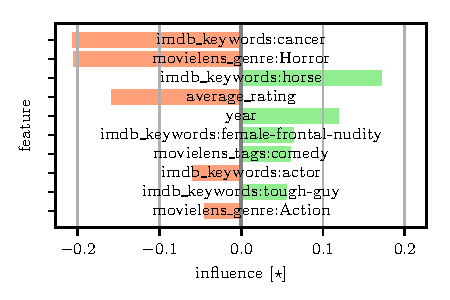
\includegraphics[width=3in]{figures/qii_user_7_movie_2713_real_data.pdf}
    \caption{User 7's recommendation about Lake Placid (1999)}
  \end{subfigure}~
  \begin{subfigure}[t]{0.45\textwidth}
    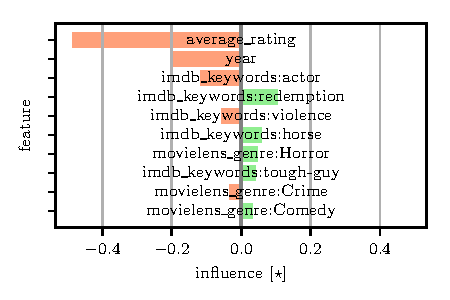
\includegraphics[width=3in]{figures/qii_user_21_movie_2713_real_data.pdf}
    \caption{User 21's recommendation about Lake Placid (1999)}
  \end{subfigure}

  \begin{subfigure}[t]{0.45\textwidth}
    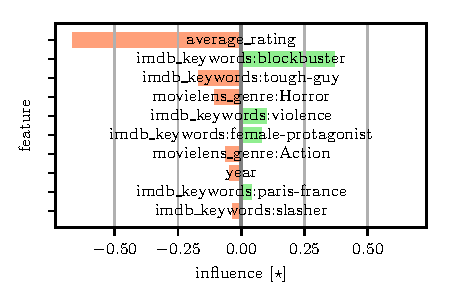
\includegraphics[width=3in]{figures/qii_user_7_movie_2720_real_data.pdf}
    \caption{User 7's recommendation about Inspector Gadget (1999)}
  \end{subfigure} ~
  \begin{subfigure}[t]{0.45\textwidth}
    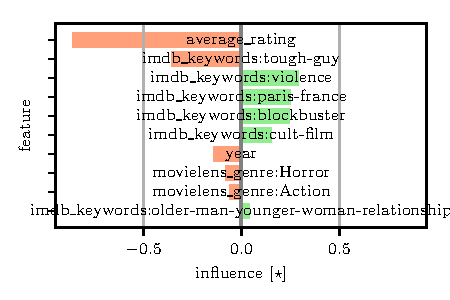
\includegraphics[width=3in]{figures/qii_user_21_movie_2720_real_data.pdf}
    \caption{User 21's recommendation about Inspector Gadget (1999)}
  \end{subfigure}


  \caption{\label{fig:results:qii}A sampling of QII-based
    recommendation interpretations based on shadow models over the
    MovieLens 20M dataset for User 7 (left) and User 21 (right).
  }
\end{figure*}


We measure the quality of the shadow model by computing the mean
absolute error of its predictions compared to the original model,
that we call \emph{baseline}.

Another metric of the quality of the shadow model is how close it
agrees with the original model on the latent factors themselves.
For each factor, we compute the mean absolute error (MAE) of latent
factor prediction. 
Averaging over all factors, we get a measure of the overall latent
factor agreement.

In our experiments, we used all movie ratings from MovieLens 20M dataset for constructing
a recommender system. 
For subsequent steps, however, we performed several pre-processing
steps.

Our implementation is based on a set of Python programs that make use
of the Apache Spark library for model training and evaluation.

We encode nominal features via one-hot encoding, and in a feature
selection step, we dropped those not meeting a minimal entropy
threshold.
For training and evaluating explanations, we also pruned away movies
with missing or negligible metadata. 
We justify this step as a deployed recommendation explanation system
could itself recognize its lack of metadata and notify users of said
fact instead of providing a potentially inaccurate explanation for its
recommendation.

The MovieLens ratings constituted the sparse user-item input matrix
for the training of a recommender system.
This data is also the \emph{ground truth} for evaluation purposes
later in this section.
The ground truth was processed with alternating least squares matrix
factorization algorithm, as implemented in Apache Spark MLlib, which
outputs two matrices: \emph{user features} and \emph{movie features},
which encode user preferences and movie properties along
low-dimensional space of \emph{latent features}. 

We trained recommender systems, constructed shadow models, and
measured the prediction error of both individual
latent factors (which can be then averaged across all of them)
and the overall predicted ratings, iterating over
several possible parameters (rank and regularization parameter for the
recommender, type of the shadow model (linear or decision tree), and
the number of bins and maximal depths for tree models). The results of
these experiments are summarized in Figure
\ref{table:results:parameters}.

\begin{figure}
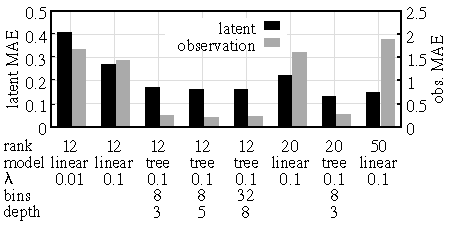
\includegraphics[width=\textwidth]{figures/shadow_parameters_accuracy.pdf}
\caption{\label{table:results:parameters} Mean absolute error of shadow
	models compared to real models with different parameters. Two metrics
	are shown: error in predicting latent factors of the real model, and error
	in predicting the ratings the real model gives}
\end{figure}

It can be seen that linear models consistently perform worse on both
metrics than decision trees. 
However, the difference in performance is much higher on observational
agreement than on latent factor agreement. 
We hypothesize that it could be due to to the linear regression models
having a consistent bias that adds up during the matrix multiplication
which is consistent with our
observations.

The observational agreement for linear models also gets worse with higher ranks,
whereas the latent factor agreement gets better, which is also consistent with the
bias hypothesis.

In our experiments, one model (Rank 50, tree, lambda 0.1, depth 5, bins 32) performed
best on both metrics, but in general, there can be a trade-off between them. Namely,
if we exclude the best-performing model, we can see that different models are the
second-best for latent factor agreement (rank 20, tree, lambda 0.1, 8 bins, depth 3)
and observational agreement (Rank 12, tree, lambda 0.1, 8 bins, depth 5),
although their performance is reasonably close to each other.











One piece of proposed work is to apply this method to course recommendations by
Coursera, with whom we are discussing the possibility of collaboration. The
usage of a recommendation system with good transparency properties could improve
both how much the users trust the system and how good the recommendations
given to them are.
